\documentclass[letterpaper,fleqn]{article}
\usepackage[final,nonatbib]{NIPS}
%\usepackage[nomarginpar,margin=0.75in]{geometry}
\usepackage{mathtools,amsthm,amssymb}
\usepackage{mathrsfs,dsfont}
\usepackage{cancel,setspace}
\usepackage{ulem, csquotes}
\usepackage{fancyhdr,hyperref}
\usepackage[usenames,dvipsnames]{color}
\usepackage{collectbox}
\usepackage{algorithm,algorithmic}
\usepackage{relsize,graphicx,subfig}
\usepackage[style=numeric,url=false]{biblatex}

\allowdisplaybreaks

\MakeOuterQuote{"}

% \pagestyle{fancy}{
% \fancyhf{}
% \lfoot{\today} 
% \cfoot{Lieberman}
% \rfoot{Page \thepage}
% }
% \renewcommand{\headrulewidth}{0pt}
% \renewcommand{\footrulewidth}{0.1pt}

% \advance\footskip 0.4cm
% \advance\textheight -0.4cm
% \calclayout

\setlength{\parindent}{0in}

\urlstyle{same}
\definecolor{darkblue}{RGB}{0,50,130}

\theoremstyle{plain}
\newtheorem{theorem}{Theorem}[subsection]
\newtheorem{lemma}[theorem]{Lemma}
\newtheorem{proposition}[theorem]{Proposition}
\newtheorem{corollary}[theorem]{Corollary}

\theoremstyle{definition} 
\newtheorem{remark}[subsection]{Remark}
\newtheorem{definition}[subsection]{Definition}


\makeatletter
\newcommand{\mybox}{%
    \collectbox{%
        \setlength{\fboxsep}{1pt}%
        \fbox{\BOXCONTENT}%
    }%
}
\makeatother

\renewcommand{\qedsymbol}{$\blacksquare$}
\newcommand{\dd}[1]{\mathop{}\!\mathrm{d}#1}
\newcommand{\Prob}[1]{\mathbb{P} \left(#1\right)}
\newcommand{\1}{\mathds{1}}

\addbibresource{references.bib}


\title{Low-Dimensional Filamentary Structures}

\author{%
  David Lieberman \\
  Department of Statistics and Data Science \\
  Yale University \\
  \href{mailto:david.lieberman@yale.edu}{\texttt{david.lieberman@yale.edu}} \\
}
\begin{document}

\maketitle

\begin{abstract}
    Often multivariate data has an intrinsic lower dimensional structure that may be illustrative of more fundamental relationships. This underlying structure may be exploited in the fields of statistical inference, clustering, and dimensionality reduction. One such structure is a "filament" — a local maximizer of the density in the normal direction as defined by the Hessian. In this paper, we first describe the Kernel Density Estimator Subspace Constrained Mean-Shift (KDE-SCMS) algorithm as a means of extracting filaments, then apply this algorithm to real data. First, to a known California earthquakes data set as a proof-of-concept, then to a novel COVID data set as a means of exploring the virus' spread across the continental United States. Finally, we explore a possible refinement of the algorithm using nearest-neighbors as a potential speed-up by locally approximating the Hessian.
\end{abstract}

\section{Background}

In general, the local maxima of a function $f(x)$ in the direction of a vector $a$ is given by the set of points $x$ such that:
$$a^T \nabla f(x) = 0, \quad a^T \mathrm{H}f(x)a < 0$$

\begin{definition}
A \textit{ridge point} is one for which:
$$V(x) V(x)^T \nabla f(x) = 0 \quad \text{AND} \quad V(x)^T \mathrm{H}f(x) V(x) < 0$$
with V(x) taken to be the second eigenvector of H$f(x)$ corresponding to the second lowest energy eigenvector $\lambda_2$. Note: the quadratic form with the Hessian being negative implies all eigenvalues of H$f(x)$ are negative.
\end{definition}

\begin{remark}
Note that in the gradient expression, the left hand side $V(x) V(x)^T \nabla f(x)$ has the interpretation that the “projected gradient” (the gradient in the direction of the normal) is zero, so $x$ lies in the tangent space and one of the eigenvectors of the Hessian is parallel with the gradient. In the Hessian expression, we see that the eigenvalues in the normal space must all be negative. In other words, the ridge is a local maximizer of the density when moving in the normal direction defined by the Hessian.
\end{remark}

\begin{definition}
A \textit{filament} is simply the set of ridge points of a smooth function (for our purposes a PDF) where the eigengap $\lambda_1(x) - \lambda_2(x) > 0$ (this is ensured as the eigenvalues of the Hessian are all negative, and $\lvert \lambda_2 \rvert  > \lvert \lambda_1 \rvert$). Thus, filaments are smooth low-dimensional structures with high density.
\end{definition}

\textbf{Context.} The concept of a filament and the methods described herein for finding them take inspiration from prior clustering techniques of maximum likelihood. The points of the filament are by construction a subset of the local maxima of the PDF. Thus, we may employ a modified version of the mean-shift algorithm already widely used in clustering, and just add the additional constraint that these points must also be maxima in the tangent space.

\quad So far, filament techniques have been almost exclusively applied in the context of cosmological data to study filamentary star structures in galaxies. Below, we validate the Kernel Density Estimator Subspace Constrained Mean-Shift algorithm (KDE-SCMS) against known results on the canonical California earthquakes geospacial data set, before applying it to the COVID-19 time-series data published by Johns Hopkins as a means of tracking path of spread of the coronavirus across America.

\section{Filament Estimation and Validation}
\subsection{KDE-SCMS}
From a high-level, the Kernel Density Estimator Subspace Constrained Mean-Shift (KDE-SCMS) algorithm, can be understood as having two main steps:

\begin{enumerate}
    \item First, compute the Kernel Density Estimator at every point, filtering out points in low-density regions below a threshold hyper-parameter $\tau$. This step essentially performs a de-noising of the data to ensure we don't end up with isolated points in low density regions which are too far from the pack to have perturbations strong enough to iteratively converge towards the maxima in the next step.
    \item Second, perform the subspace constrained mean-shift algorithm to converge to the local maxima, iteratively. This step essentially performs a modified gradient ascent using a kernel function.
\end{enumerate}

\mbox{}

The Step (1) was first introduced by Wasserman in \cite{SuRF}, so we denote KDE-SCMS(V1) as \textbf{without} thresholding, and KDE-SCMS(V2) as \textbf{with} thresholding. 

Below we visualize the impact of thresholding our data using a random sample of 4000 observations from the California earthquakes data set as a reference point:

\begin{figure}[!htb]
    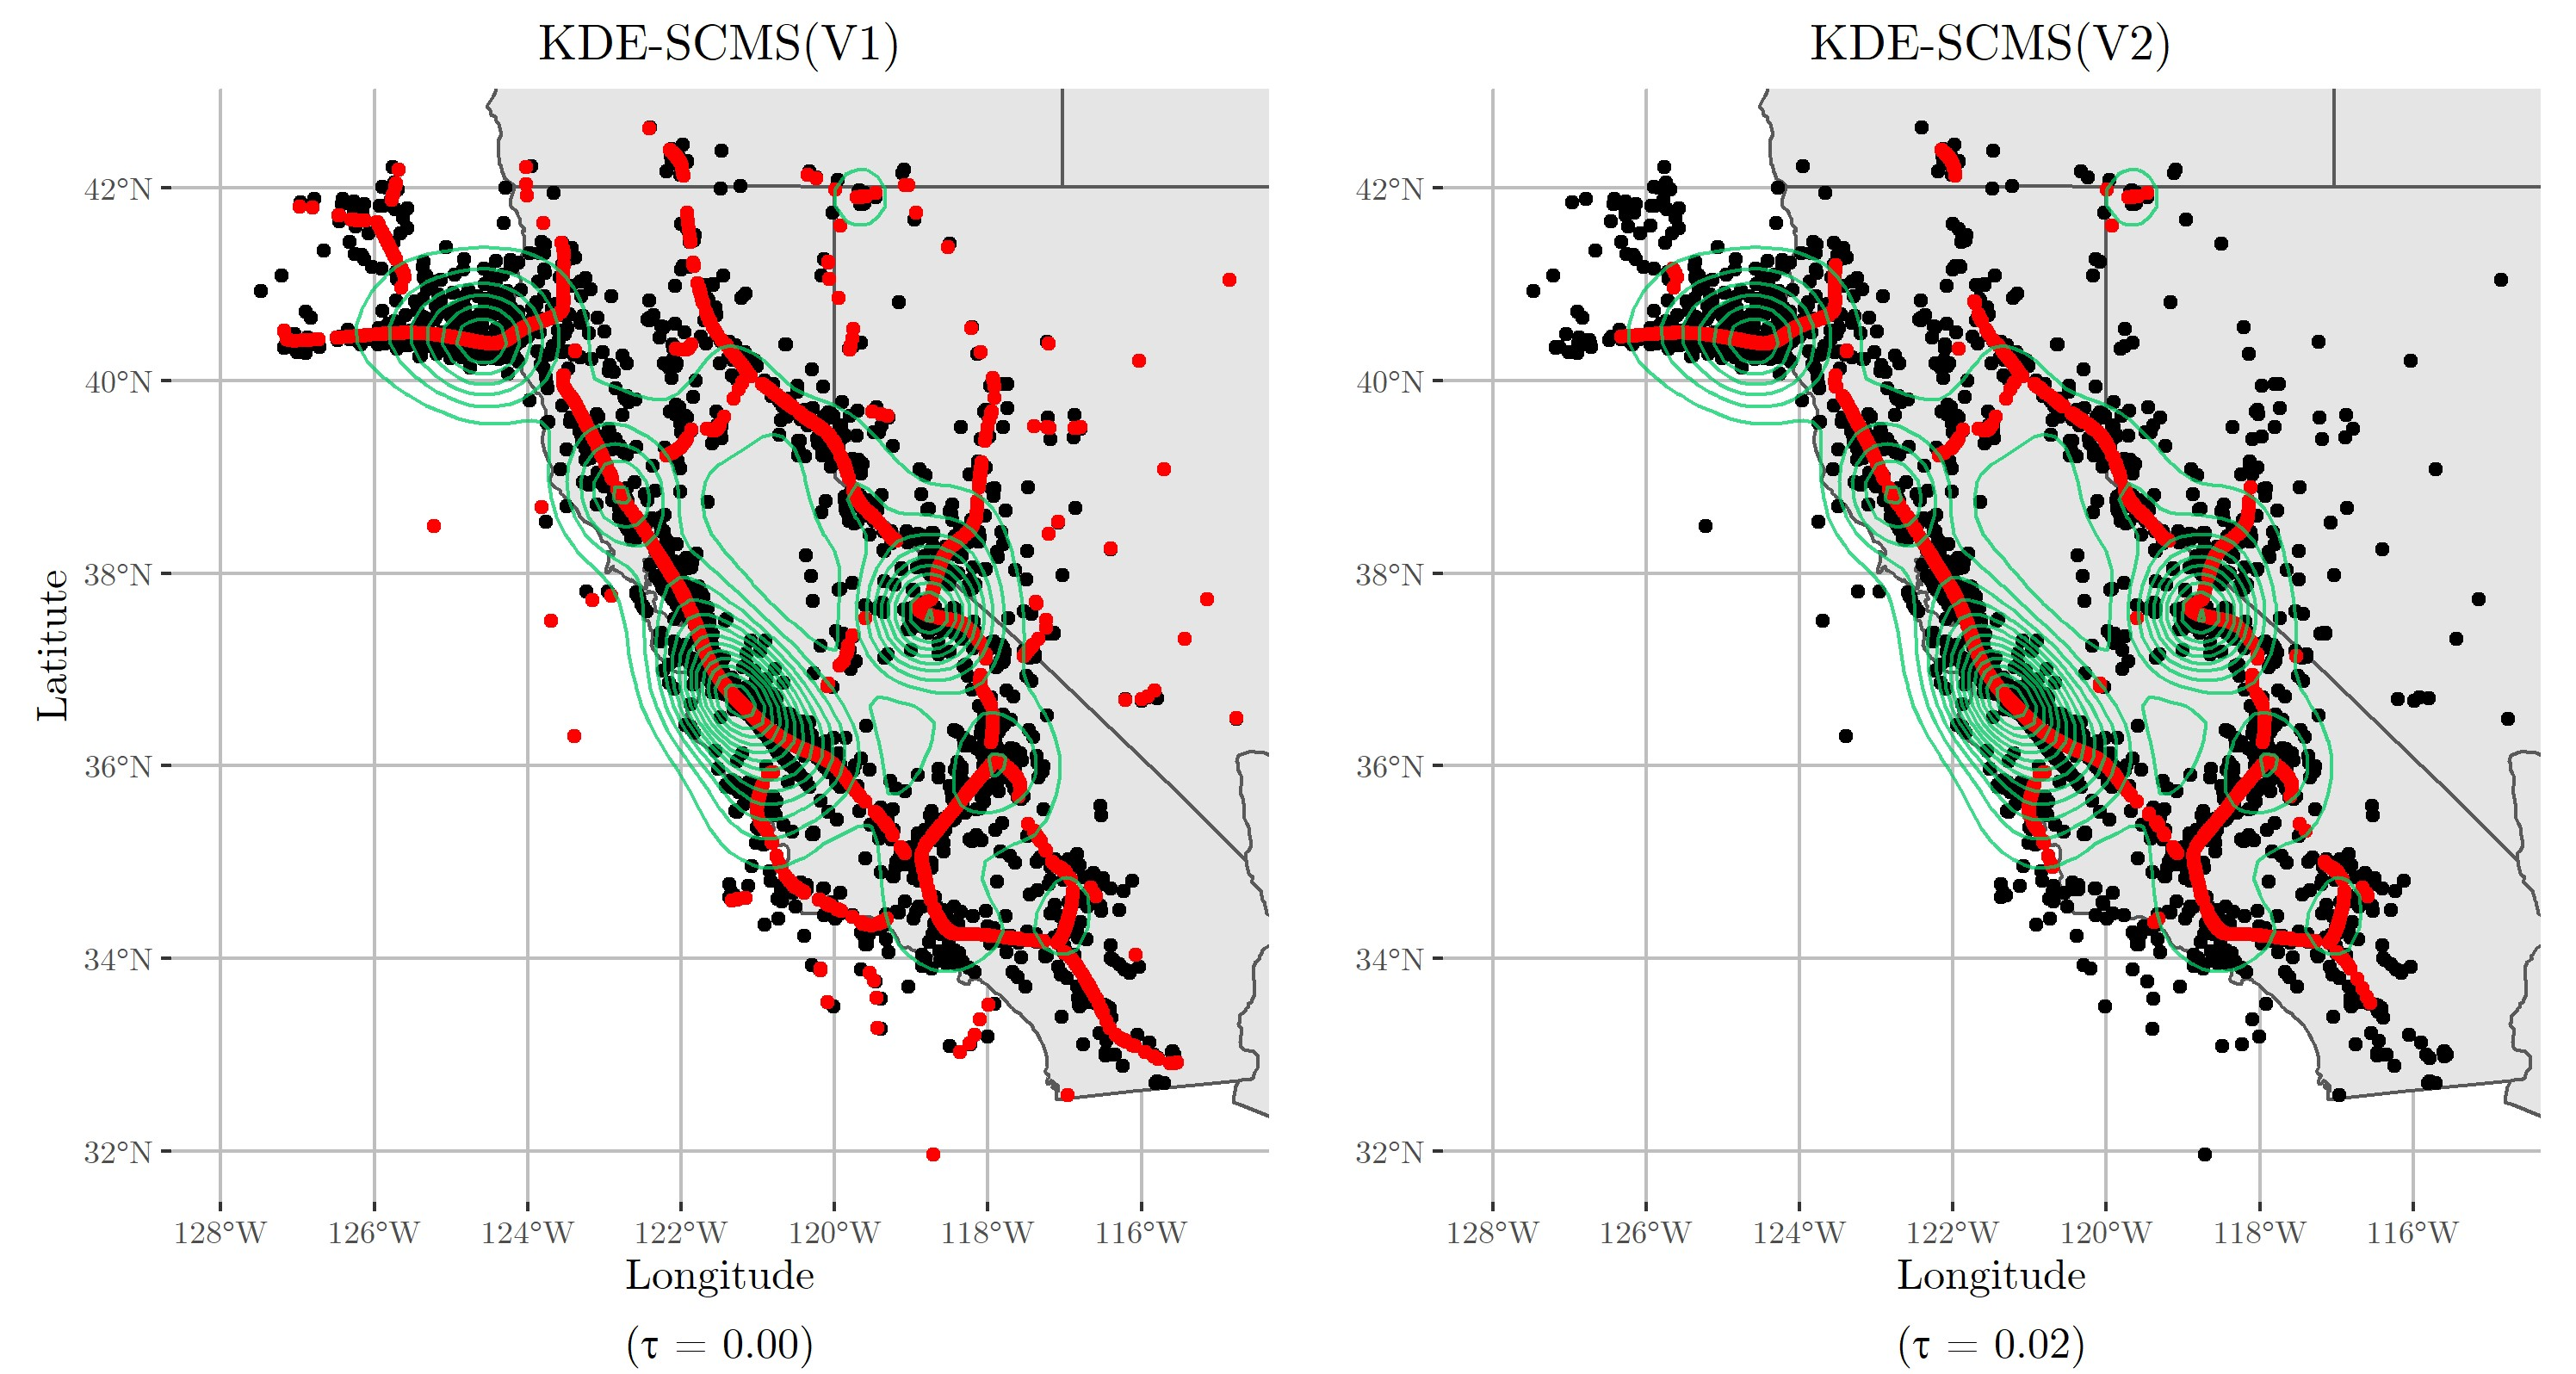
\includegraphics[width=\textwidth]{combined.jpg}
    \caption{Black = Input Data; Red = Converged Filament Set; Green-Bands = Contour Lines of KDE}%
    \label{fig:thresholding}%
\end{figure}

\newpage

Unsurprisingly, but excitingly nonetheless, the filamentary structure here actually finds the fault lines in California from just the locations of the earthquakes alone.

\begin{figure}[!htb]
    \centering
    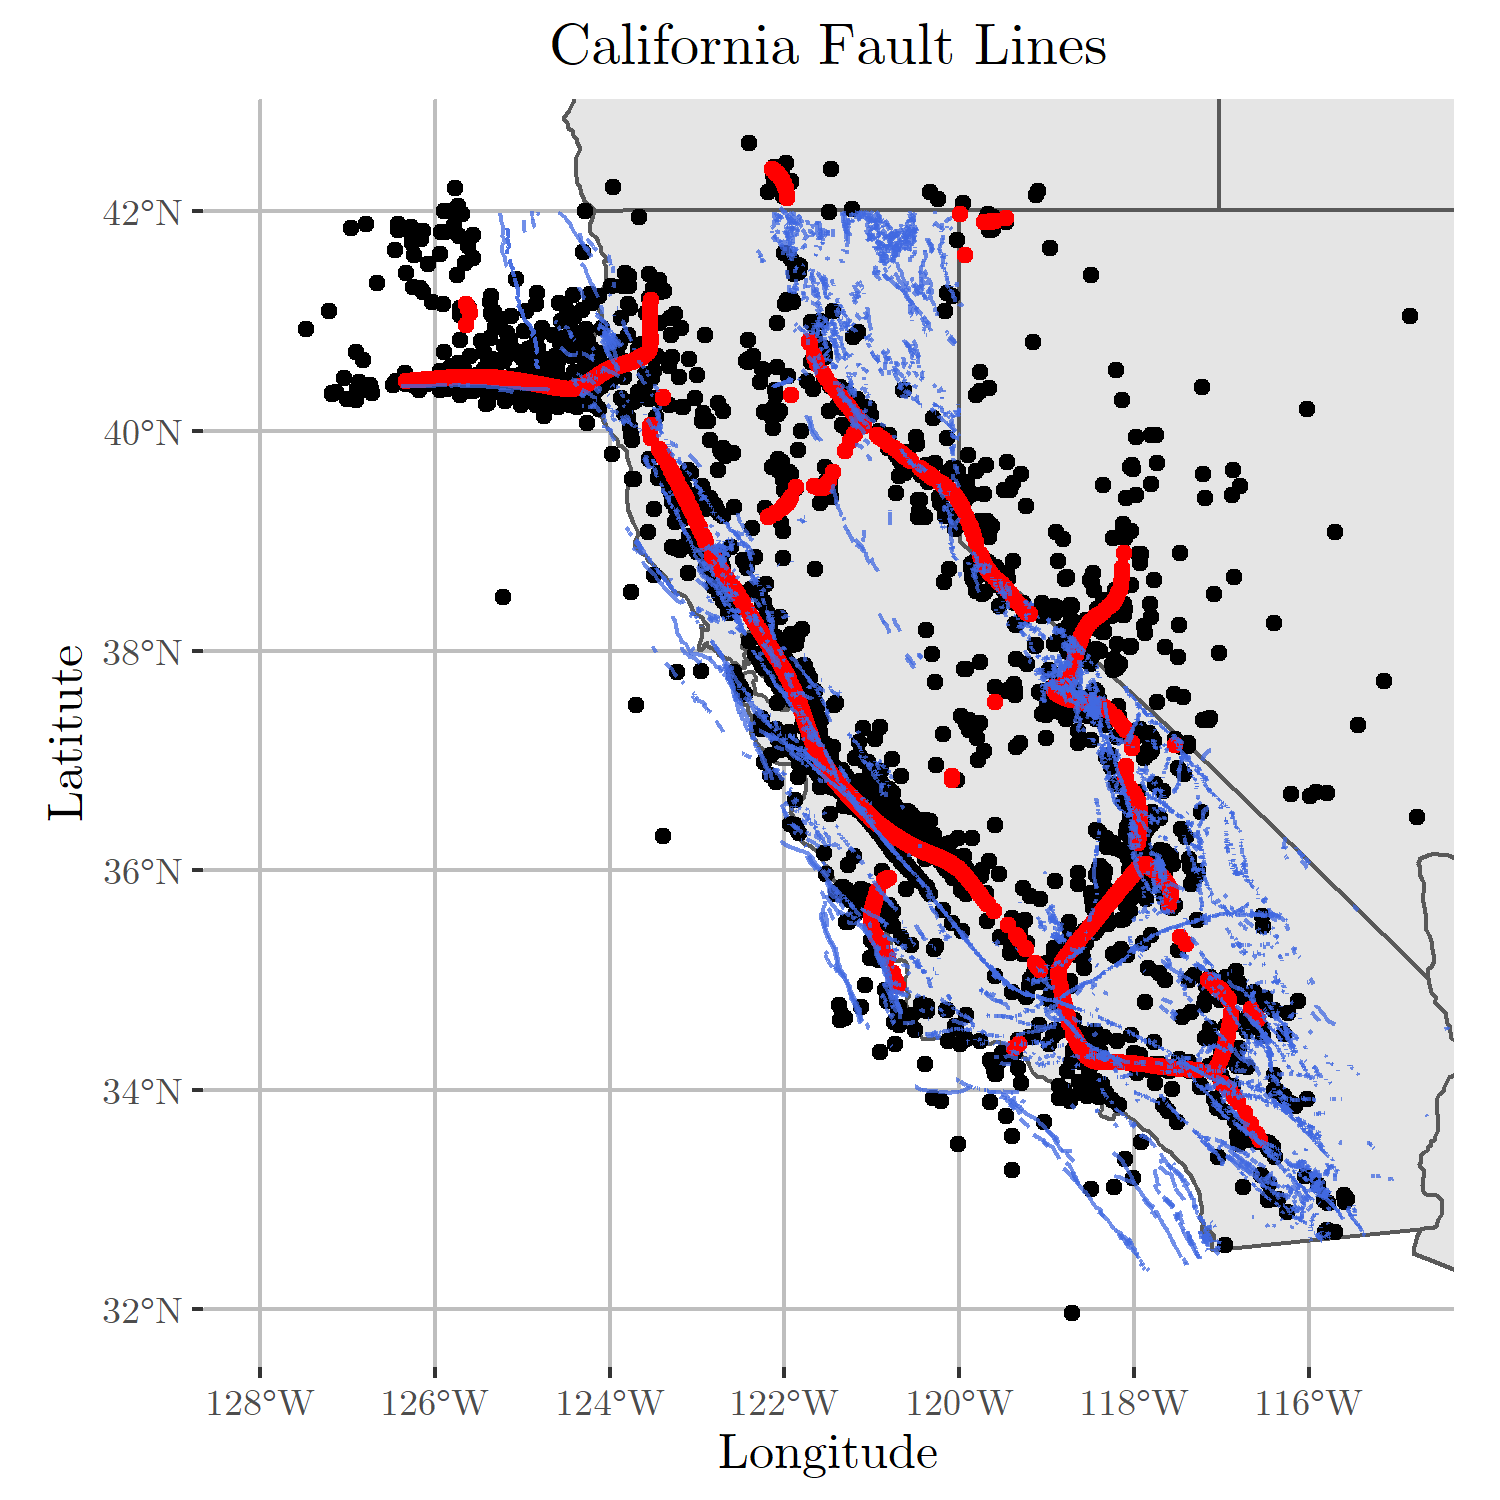
\includegraphics[width=0.65\textwidth]{faults_overlay.png}
    \caption{Black = Input Data; Red = Converged Filament Set; Blue-Traces = California Fault-lines (obtained via USGS.gov GIS)}%
    \label{fig:faultlines}%
\end{figure}


\newpage

Now we give a more detailed description of the KDE-SCMS algorithm\cite{algo}:

\begin{algorithm}[!htb]
\setstretch{1.25}
\caption{KDE-SCMS(V2)  \textit{(Kernel Density Estimator Subspace Constrained Mean-Shift)}}
\begin{flushleft}
        \textbf{Input:} Data $\{X_1, \dots, X_n \}$. Kernel function $K(\cdot)$. Smoothing bandwidth $h$. Threshold $\tau$.\\
\end{flushleft}
\begin{algorithmic}
    \STATE \textbf{Step 1.} Compute the kernel density estimator $\hat{p}(x)$ via
        \begin{flalign*}
        \hat{p}(x) = \frac{1}{nh^d} \sum_{i=1}^{n} K\left(\frac{\lVert x - X_i \rVert}{h}\right)
        \end{flalign*}
        
    \STATE \textbf{Step 2.} Select a mesh $\mathcal{M}$ of points. By default, we can take $\mathcal{M} = \{X_1, \dots, X_n \}$.
    
    \STATE \textbf{Step 3.} Thresholding: remove $x \in \mathcal{M}$ if $\hat{p}(x) < \tau$. Denote the mesh points remaining as $\mathcal{M}'$.
    
    \STATE \textbf{Step 4.} For each $x \in \mathcal{M}'$, perform the following subspace constrained mean shift until convergence:
    
    \begin{ALC@g}
         \STATE \uline{Step 4-1.} For $i = 1, \dots, n$, compute
            \begin{flalign*}
                \mu_i = \frac{x - X_i}{h^2}, \quad c_i = K\left(\frac{x - X_i}{h}\right)
            \end{flalign*}
            
         \STATE \uline{Step 4-2.} Compute the Hessian matrix
            \begin{flalign*}
                \mathrm{H}(x) = \frac{1}{n} \sum_{i=1}^{n} c_i \left(\mu_i \mu_i^{T} - \frac{1}{h^2}\mathbf{I}\right)
            \end{flalign*}
            \vspace{-0.75em}
        \STATE \uline{Step 4-3.} Perform spectral decomposition on $\mathrm{H}(X)$ and compute $V(x) = [v_2(x), \dots, v_d(x)]$, the eigenvectors corresponding to the smallest $d-1$ eigenvalues.
        \STATE \uline{Step 4-4.} Update $x \rightarrow V(x)V(x)^{T}m(x) + x$ until convergence, where
            \begin{flalign*}
                m(x) = \frac{\sum_{i=1}^{n} c_i X_i}{\sum_{i=1}^{n} c_i} - x
            \end{flalign*}
        is called the mean-shift vector.
        \STATE \uline{Step 4-5.} \textbf{Terminate} when $\Vert m(x) \Vert < \epsilon$.
    \end{ALC@g}
\end{algorithmic}
\begin{flushleft}
    \textbf{Output:} The collection of all remaining points\\
\end{flushleft}
\end{algorithm}

We note that this algorithm has time complexity issues with run-time $O(N^2 d^3)$ where N is the number of points and d is the dimension, as we are performing a double for-loop: outside for-loop running over all the points (parallelizable!), while the inside for-loop calculates the update perturbation for a single point by taking the kernel function over all other points. Note that the mean-shift vector $m(x)$ is essentially our estimator for the gradient of the PDF $\nabla f(x)$ as originally described on page 1. We want this matrix quantity to converge to the zero vector, so our termination criteria is $\Vert m(x) \Vert < \epsilon$.

\newpage

\section{Application}

We thought it might be feasible to try and use the KDE-SCMS to track the spread of COVID across the United States, as the virus is highly contagious so density of cases serve as a good heuristic for path of transmission. We used Johns Hopkins' COVID-19 time-series data\cite{covid_data} which gives the number of COVID confirmed cases, by county. As we wanted to make sure data was not singular, we repeated the latitude and longitude coordinates of a point by the number of cases and added a small amount of noise. This is a realistic modification as people from around the county are not isolated at a single point and live proximal to one another. We provide an interactive visualization of our data \href{https://kepler.gl/demo/map?mapUrl=https://dl.dropboxusercontent.com/s/tmpj2dkr0w1vhoj/keplergl_7k43a5f.json}{\textcolor{darkblue}{here}}.

Here are some initial time-series results we obtained through KDE-SCMS:

\vspace{-1em}
\begin{figure}[!htb]
  \makebox[\textwidth][c]{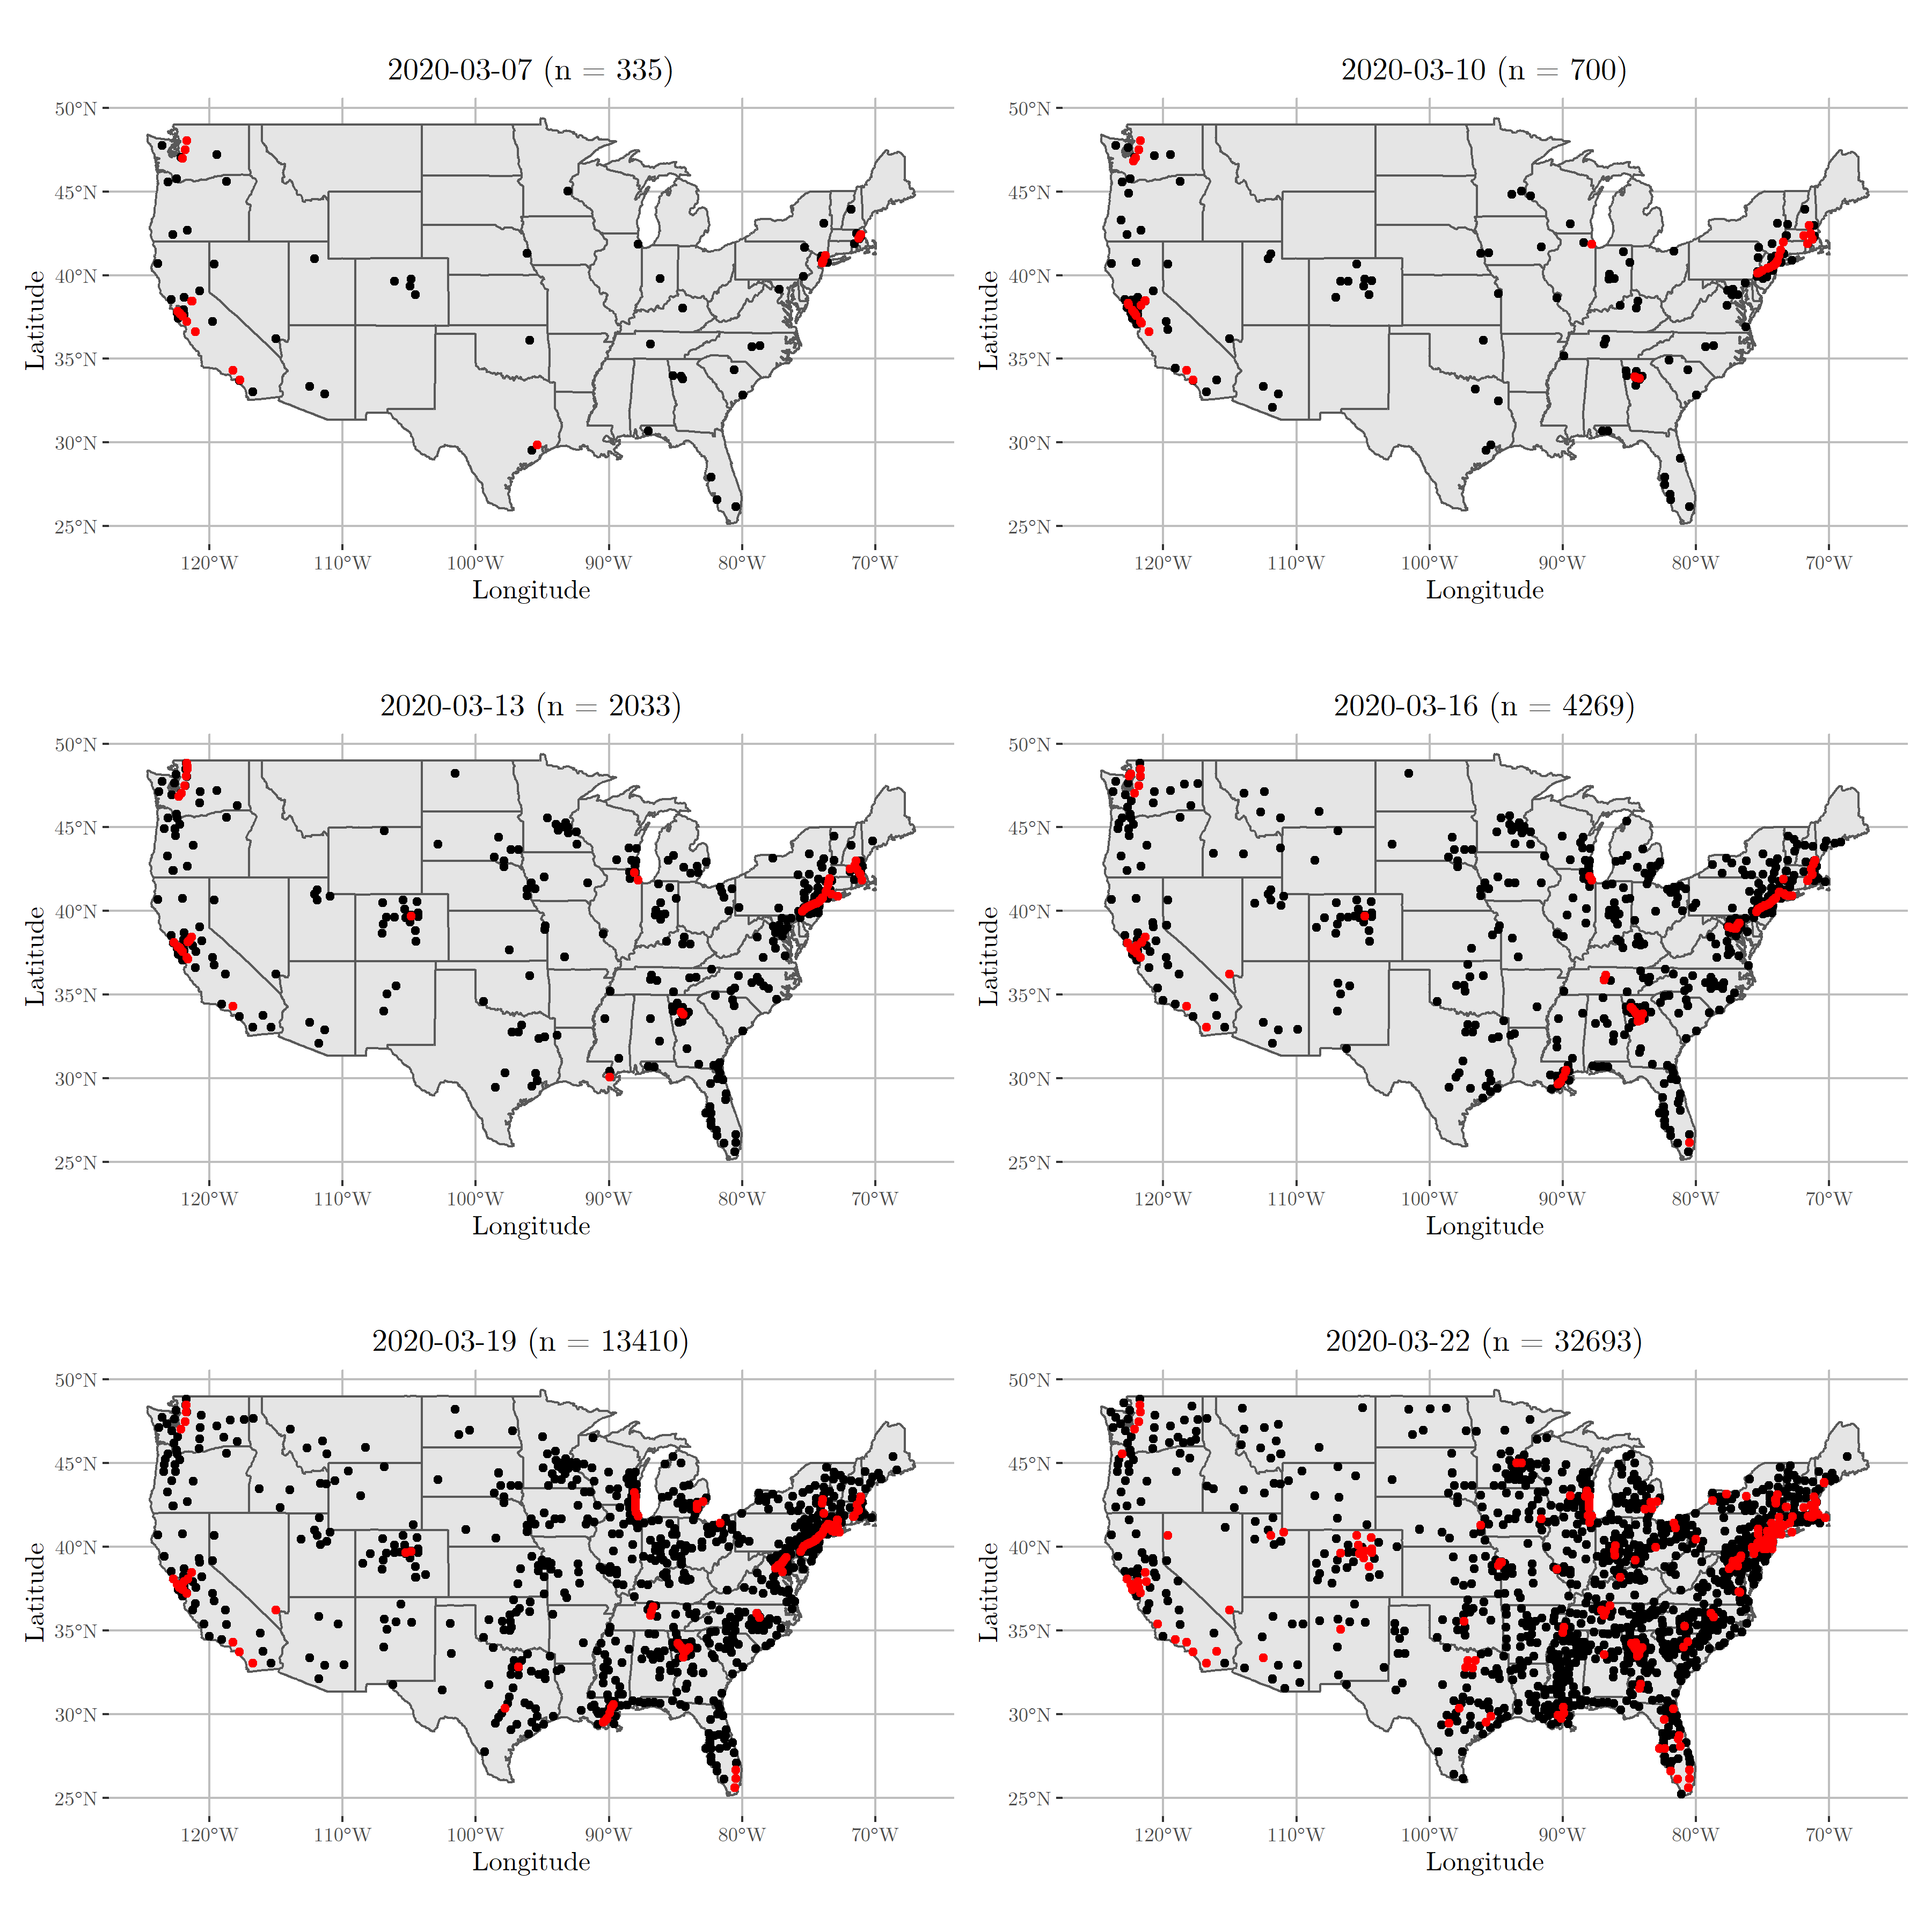
\includegraphics[width=1.25\textwidth]{COVID_timeseries.png}}%
\end{figure}
\vspace{-1em}
(See \href{https://github.com/davidlieberman/AMATH797/tree/master/Project}{\textcolor{darkblue}{supplementary C++ code}} for our implementation)

\newpage

\begin{figure}[!htb]
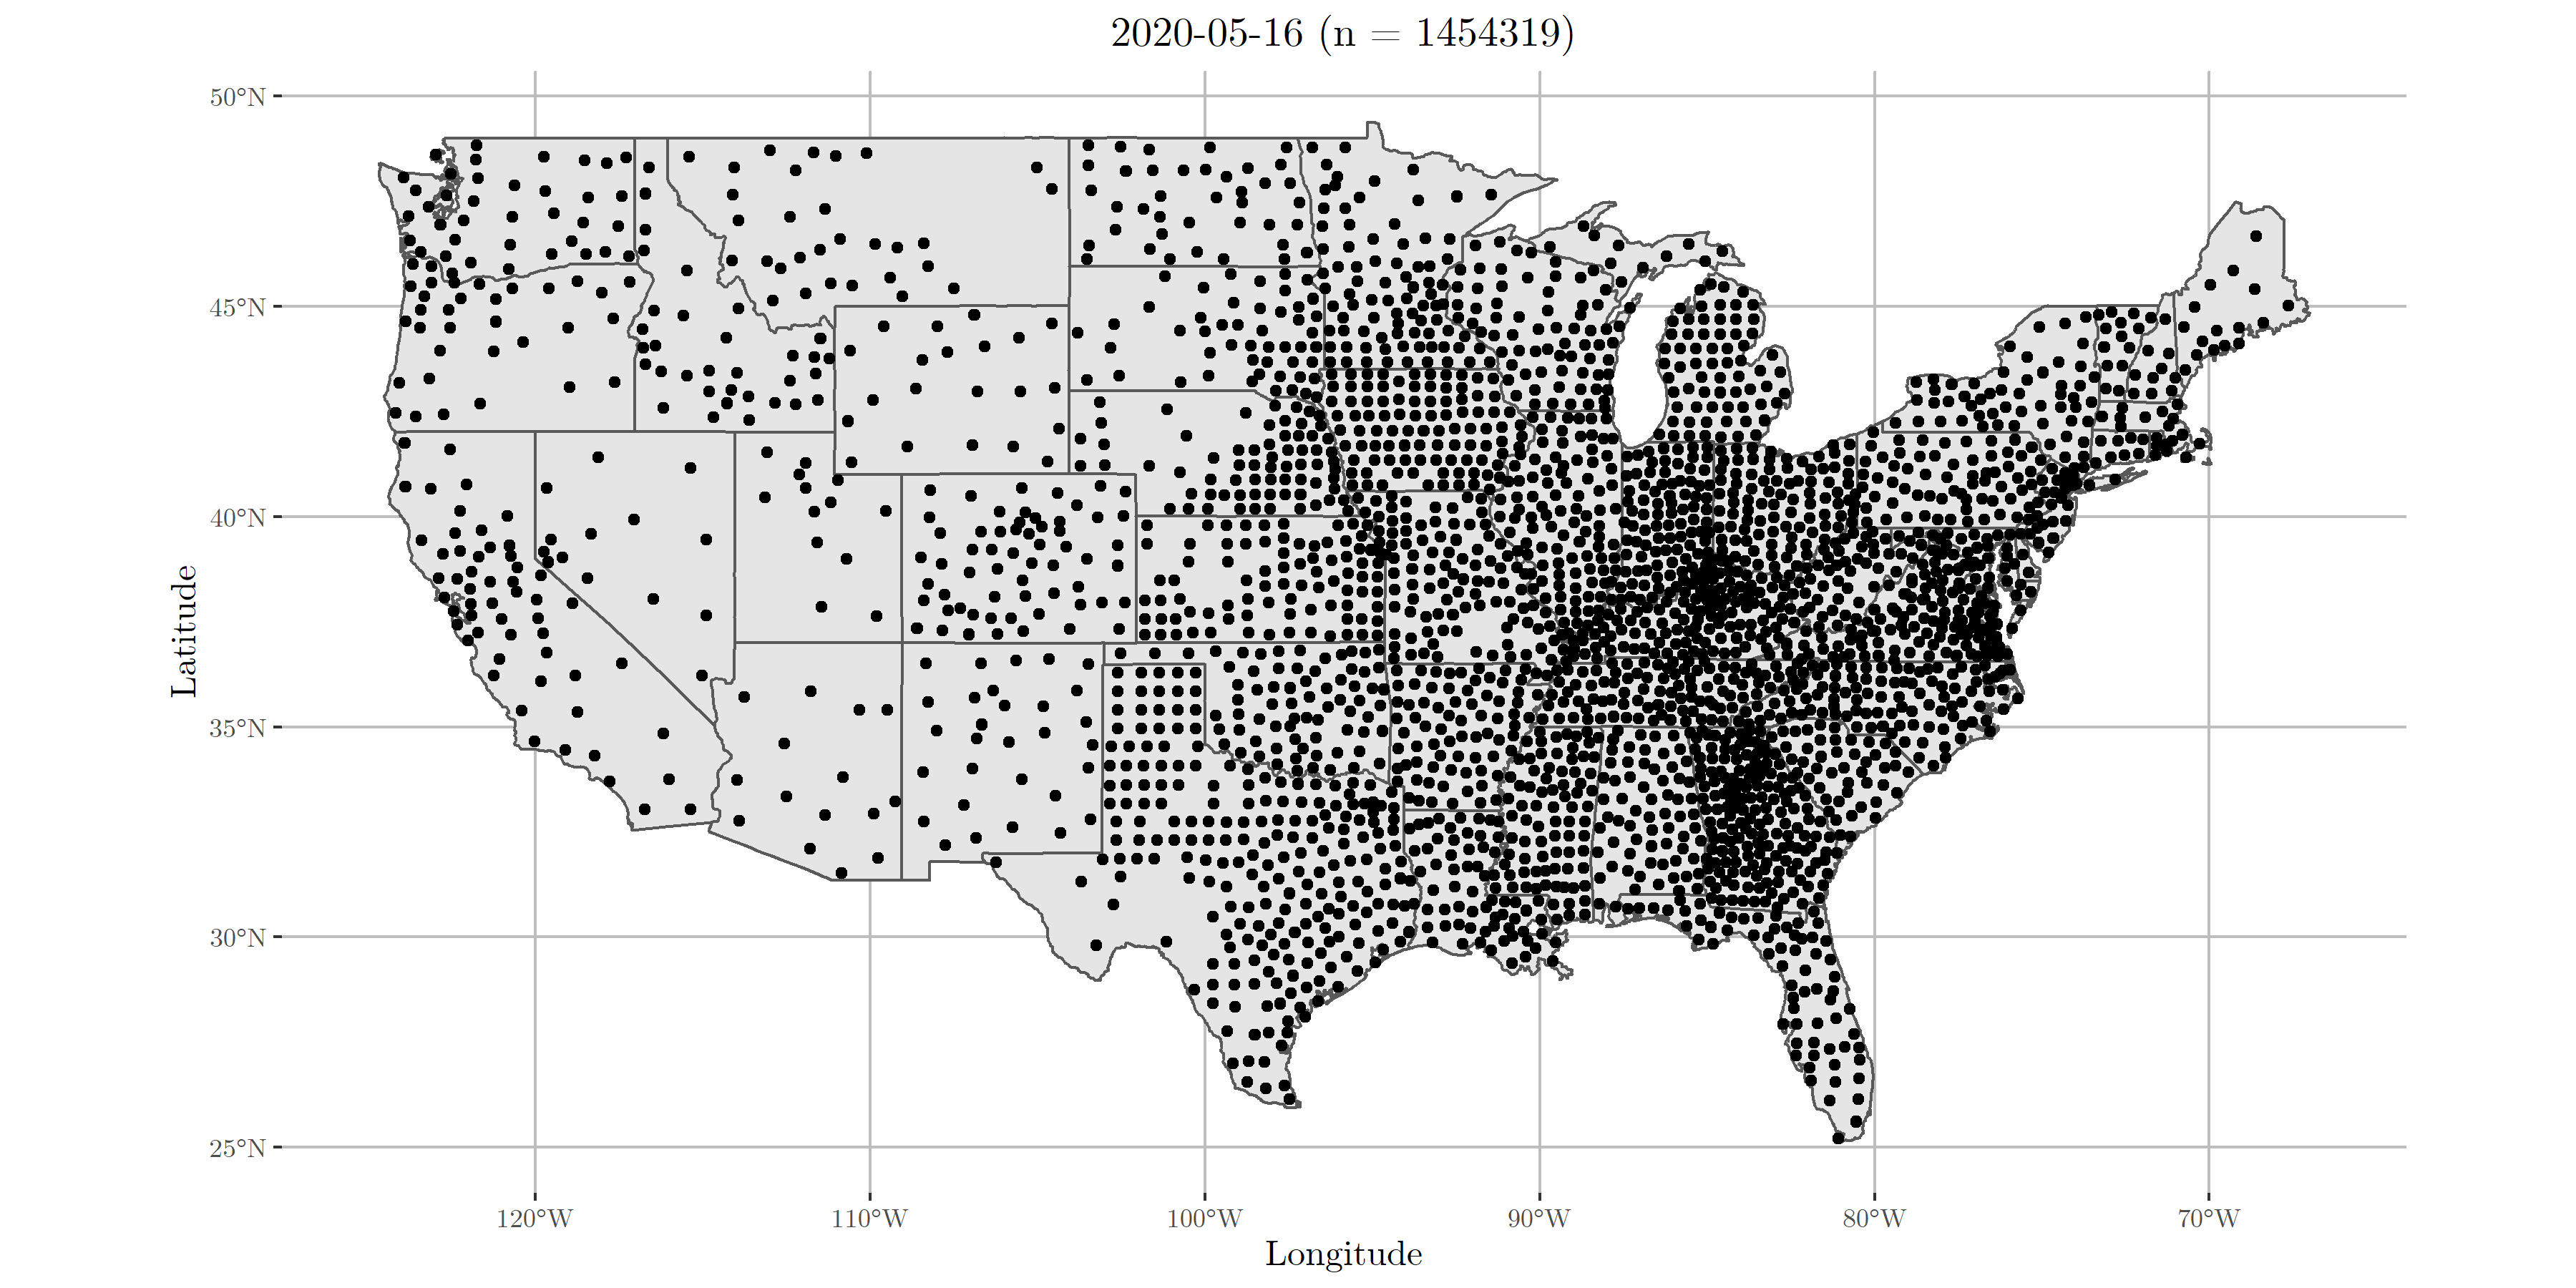
\includegraphics[width=\textwidth]{millions.png}
\end{figure}

Unfortunately, as N tends towards a million and a half, the run-time goes up dramatically and KDE-SCMS becomes totally infeasible without significant further optimizations. We first implemented a modified KDE-SMCS using nearest-neighbors, calculating the approximate local Hessian using only points within 3 standard deviations away (i.e. 3 times the kernel bandwidth, which approximates this when chosen well), rather than summing over the whole data set. The first way we implemented the nearest-neighbors algorithm was using the KD-Tree method, which, while it did reduce the summation computations, the nearest-neighbors algorithm itself required a non-trivial amount of compute resources. As a result, we also explored using an approximate nearest-neighbors method by Yashunin\cite{hnsw}, which uses hierarchical navigable small world graphs to efficiently and quickly compute neighbors, even on large data sets. However, it seems that the benefit is most had on data that suffers from the "Curse of Dimensionality" — potentially beneficial for KDE-SMCS run on high-dimensional data sets — but not for our $\mathbb{R}^2$ data here. It is worth noting that implementing these nearest-neighbor approximations came at no noticeable decrease in accuracy of the method. However, we remain unable to compute KDE-SCMS on data sets with greater than 50 thousand points. Hopefully, more to come soon.

\newpage
\nocite{*}
\printbibliography

\end{document}